% !TEX root = ../Thesis.tex

\chapter{Polimorfismo}
Il polimorfismo è un concetto fondamentale della programmazione. Derivato dal greco “molte forme”, il polimorfismo consente a entità di assumere diverse forme o comportamenti in base al contesto, permettendo di scrivere codice più flessibile, estendibile e manutenibile. Grazie al polimorfismo, è possibile utilizzare un'interfaccia comune per manipolare elementi di tipi diversi, facilitando così l'implementazione di soluzioni generiche. Il vantaggio principale del polimorfismo è il miglioramento della qualità del codice:
\begin{itemize}
    \item Favorisce l'astrazione, consentendo di trattare oggetti di tipi diversi in modo uniforme.
    \item Riduce la duplicazione di codice, poiché le operazioni comuni possono essere definite una sola volta e riutilizzate per diversi tipi.
    \item Semplifica la gestione delle estensioni future, poiché nuove funzionalità possono essere aggiunte senza modificare il codice esistente.
\end{itemize}
In un linguaggio come Java, orientato agli oggetti, il polimorfismo è una caratteristica centrale e largamente supportata tramite ereditarietà e interfacce. Rust, pur non essendo un linguaggio tradizionalmente orientato agli oggetti, offre un approccio alternativo al polimorfismo, basato su trait e tipi generici, che permette di ottenere astrazione e flessibilità.

In particolare, quando il codice coinvolge il polimorfismo, sono necessari meccanismi per determinare quale versione specifica di metodo sta venendo effettivamente eseguita. Questo processo prende il nome di \textit{dispatch}. Esistono due forme di dispatch: 
\begin{itemize}
    \item Lo \textit{Static Dispatch}, in cui la risoluzione della chiamata viene risolta a tempo di compilazione.
    \item Il \textit{Dynamic Dispatch}, in cui la risoluzione della chiamata avviene a run-time. 
\end{itemize}
In questo capitolo verrà fornita una panoramica delle modalità con cui Java e Rust forniscono supporto al polimorfismo, confrontando i due linguaggi.
\section{Polimorfismo in Java}
Java supporta il polimorfismo attraverso due principali meccanismi: il \textit{subtyping} (polimorfismo per inclusione) e il \textit{parametric polymorphism} (polimorfismo parametrico). 

Il subtyping si basa sul fatto che ci possa essere una relazione tra tipi chiamata \textit{relazione di sottotipo}. Si dice che un tipo \textit{A} è un sottotipo di un tipo \textit{B} quando il contesto richiede un elemento di tipo \textit{B} ma può accettare un elemento di tipo \textit{A}. In Java, la relazione di sottotipo viene implementata attraverso l'ereditarietà e le interfacce. Le classi possono estendere altre classi e implementare interfacce, consentendo agli oggetti di essere trattati come istanze della loro classe base o interfaccia. 

Il parametric polymorphism permette di assegnare a una parte di codice un tipo generico, utilizzando variabili di tipo al posto di tipi specifici, che poi possono essere istanziate con tipi concreti al momento dell'utilizzo. In particolare, Java supporta l'\textit{F-bounded polymorphism} \cite{greenman-effing-bound-polymorphism}, che è la capacità di poter definire vincoli su un tipo generico che possono anche essere ricorsivi. Ad esempio \texttt{<T extends Comparable<T>}\texttt{>}.

\section{Polimorfismo in Rust}
In Rust, il polimorfismo è implementato attraverso i concetti di \textit{trait} e i \textit{generics}. I trait sono simili alle interfacce in Java e definiscono un insieme di metodi che un tipo deve implementare per essere considerato conforme a quel trait. I generics consentono di scrivere funzioni e strutture dati che possono operare su tipi diversi senza dover specificare un tipo concreto. Tramite l'uso dei generics si ottiene il \textit{parametric polymorphism}, mentre attraverso i trait si ottiene il \textit{bounded parametric polymorphism}.\footnote{Entrambe le forme di polimorfismo hanno la stessa definizione data in precedenza per Java.}

\section{Generics: Monomorphization e Type Erasure}
\label{sec:generics}
Sia Rust che Java supportano la programmazione generica, che consente di scrivere codice che può operare su tipi diversi senza avere codice duplicato per ogni tipo specifico. La sintassi per definire i generics in Rust e Java è simile: si utilizzano parentesi angolari per specificare i parametri di tipo. Tuttavia, ci sono differenze significative nella gestione dei generics tra i due linguaggi.

Il compilatore Java utilizza un processo chiamato \textit{type erasure} per implementare i generics, questo include i seguenti fatti:
\begin{itemize}
    \item Durante la compilazione i parametri di tipo vengono sostituiti con il tipo \texttt{Object} o con un tipo specifico se è stato definito un vincolo sul parametro di tipo.
    \item Vengono inseriti cast espliciti per mantenere la type safety.
    \item Generazione di \textit{Bridge Methods} per preservare il polimorfismo dopo il processo di type erasure.
\end{itemize}
Ad esempio:
\begin{minted} [fontsize=\small] {Java}
    public class GenericClass<T> {
        T value;

        void setValue(T value) { 
            this.value = value;
        }
    }
\end{minted}
Dopo la type erasure, il codice diventa:
\begin{minted} [fontsize=\small] {Java}
    public class GenericClass {
        Object value;

        void setValue(Object value) { 
            this.value = value;
        }
    }
\end{minted}
Nel caso in cui, invece, si definisca un vincolo di tipo, ad esempio \texttt{<T extends Number>}, il compilatore Java sostituirà \texttt{T} con \texttt{Number} durante la type erasure, mantenendo la type safety:
\begin{minted} [fontsize=\small] {Java}
    public class GenericClass{
        Number value;

        void setValue(Number value) { 
            this.value = value;
        }
    }
\end{minted}
Quando si combina la type erasure con l'overriding dei metodi, Java genera dei \textit{Bridge Methods} per garantire che il polimorfismo funzioni correttamente. Uno scenario tipico è il seguente:
\begin{itemize}
    \item Una classe generica o un'interfaccia ha un metodo che usa un tipo generico. 
    \item Una sua sottoclasse sovrascrive quel metodo con un tipo concreto. 
    \item Dopo la type erasure, le firme dei due metodi non corrispondono più. Questo romperebbe il polimorfismo. 
\end{itemize}
Ad esempio: 
\begin{minted} [fontsize=\small] {Java}
    class Parent<T> {
        T getValue() { return null; }
    }

    class Child extends Parent<String> {
        @Override
        String getValue() {
             return "Hello"; 
        }
    }
\end{minted}
Dopo la type erasure:
\begin{minted} [fontsize=\small] {Java}
    class Parent {
        Object getValue() {
            return null; 
        }
    }

    class Child extends Parent {
        String getValue() {
            return "Hello"; 
        }

        // Bridge method generato dal compilatore:
        // Garantisce che la chiamata a Parent.getValue() 
        // funzioni correttamente
        Object getValue() {
            return this.getValue(); // chiama String getValue()
        }
    }
\end{minted}
In Rust, invece, i generics sono implementati tramite un processo chiamato \textit{monomorphization}. Questo è il processo tramite cui il compilatore Rust genera codice specifico per ogni tipo concreto utilizzato con i generics. Questo significa che Rust sostituisce i parametri di tipo generici con i tipi concreti utilizzati, e genera una versione specifica della funzione o della struttura per ogni tipo. Ad esempio: 
\begin{minted} [fontsize=\small] {Rust}
    struct Boxed<T> {
        value: T,
    }

    fn main() {
        let a = Boxed { value: 123 }; // T = i32
        let b = Boxed { value: "text" }; // T = &str
    }
\end{minted}
Dopo la monomorphization, il compilatore Rust genera due versioni della struttura \texttt{Boxed}:
\begin{minted} [fontsize=\small] {Rust}
    struct Boxed_i32 {
        value: i32,
    }

    struct Boxed_str {
        value: &str,
    }
\end{minted}
È facile notare come i due approcci siano molto diversi e abbiano implicazioni diverse sul modo in cui il codice viene generato e sulla performance:
\begin{itemize}
    \item Rispetto alla type erasure di Java, la monomorphization di Rust porta diversi vantaggi in termini di performance:
    \begin{itemize}
        \item Nella type erasure, poiché i parametri di tipo vengono eliminati, il compilatore spesso deve inserire cast espliciti per garantire la type safety, il che può introdurre un overhead. Questo overhead è spesso trascurabile ma comunque presente. 
        \item I generics di Java non possono essere utilizzati con tipi primitivi, come \texttt{int} o \texttt{double}, ma solo con oggetti. Questo significa che quando si usano generics con tipi primitivi, Java deve utilizzare il boxing e l'unboxing, che introducono un ulteriore overhead.
        \item Poiché Java usa lo stesso bytecode per tutte le istanziazioni di un generico, non può ottimizzare il codice per tipi specifici. Questo può essere rilevante per sistemi che richiedono un alto grado di performance.
        \item Il monomorphization è un meccanismo statico che risolve i tipi al momento della compilazione, quindi una chiamata a un metodo generico è risolta a compile time e non ci sono overhead a runtime. Invece, la type erasure può coinvolgere il dynamic dispatch di Java che può essere più costoso in termini di performance.
    \end{itemize}
    \item La monomorphization può portare ad un aumento della dimensione del codice del programma compilato poiché vengono generate diverse versioni della stessa funzione generica, una per ogni combinazione di tipi con cui viene chiamata. 
    \item La monomorphization può incrementare notevolmente il tempo di compilazione del programma, specialmente se ci sono molte combinazioni di tipi concreti con cui viene chiamata una funzione generica.
    \item La monomorphization può fornire messaggi di errore più chiari e specifici poiché ogni versione specifica della funzione generica ha tipi concreti associati.
\end{itemize}
\section{Traits}
\label{sec:rust_traits}
Un \textit{trait} è un costrutto di Rust che consente di definire un insieme di funzionalità che un tipo deve implementare. I traits vengono utilizzati, quindi, per definire comportamenti comuni che possono essere condivisi tra diversi tipi. Questo significa che tutti i tipi che implementano un determinato trait condividono la stessa interfaccia di quel trait. Un trait viene dichiarato utilizzando la keyword \texttt{trait} come segue:
\begin{minted} [fontsize=\small] {Rust}
    trait MyTrait {
        fn my_method(&self) -> ();
    }
\end{minted}
L'implementazione del trait avviene attraverso le keywords \texttt{impl} e \texttt{for} come segue:
\begin{minted} [fontsize=\small] {Rust}
    struct MyStruct;

    impl MyTrait for MyStruct {
        fn my_method(&self) -> () {
            println!("Hello from MyStruct");
        }
    }
\end{minted}
%TODO: rimosso perché spiegato nel capitolo 1
\begin{comment}
    In particolare, in Rust, il termine metodo si riferisce a una funzione definita all'interno di un blocco \texttt{impl}. Mentre per funzione si intende una funzione indipendente che viene chiamata utilizzando il suo nome seguito dagli argomenti tra parentesi (ad esempio, \texttt{function(arg1, arg2)}). Nell'esempio precedente, \texttt{my\_method()} è un metodo. Un metodo in Rust può essere chiamato utilizzando la notazione puntata, ad esempio:
\begin{minted} [fontsize=\small] {Rust}
    let obj = MyStruct;
    obj.my_method(); // Chiamata al metodo
\end{minted}
\end{comment}
I traits possono essere utilizzati per realizzare il bounded parametric polymorphism in Rust, consentendo di specificare vincoli sui tipi generici (\textit{trait bounds}). Ad esempio, si può definire una funzione che accetta un tipo generico che implementa un determinato trait nel seguente modo:
\begin{minted} [fontsize=\small] {Rust}
    fn my_function<T: MyTrait>(item: T) {
        println!("{}", item.my_method());
    }
\end{minted}
Nel caso in cui siano presenti più vincoli, questi possono essere combinati utilizzando il simbolo \texttt{+} oppure attraverso l'uso di \texttt{where}:
\begin{minted} [fontsize=\small] {Rust}
    fn my_function<T>(item: T)
    where 
        T: MyTrait + AnotherTrait 
    {
        println!("{}", item.my_method());
    }   
\end{minted}
In Java, è possibile ottenere un comportamento simile ai trait bounds attraverso i vincoli di tipo (\textit{type bounds}) nelle dichiarazioni generiche. Ad esempio, si può definire una classe generica che accetta un tipo che estende una classe base o implementa un'interfaccia:
\begin{minted} [fontsize=\small] {Java}
    public class MyClass<T extends Bound> {
        /* ... */
    }
\end{minted}
In questo esempio, \texttt{T} è un tipo generico che deve implementare \texttt{Bound}. Questo consente di utilizzare i metodi definiti in \texttt{Bound} all'interno della classe \texttt{MyClass}. Anche in Java è possibile definire più vincoli di tipo\footnote{A causa dell'ereditarietà singola di Java solo un vincolo può essere una classe: il primo nella lista.} attraverso l'utilizzo dell'operatore \texttt{\&}:
\begin{minted} [fontsize=\small] {Java}
    public class MyClass<T extends Bound & AnotherBound> {
        /* ... */ 
    }
\end{minted}
Si può facilmente notare come il concetto di trait in Rust sia molto simile alle interfacce in Java. Entrambi servono a garantire che un valore o un oggetto possa essere utilizzato secondo un certo protocollo o insieme di regole, permettendo diverse implementazioni concrete senza essere vincolati a dettagli di implementazione, a differenza di quanto accade con una superclasse Java. Inoltre, in entrambi i costrutti è possibile definire metodi di default. Tuttavia, sono presenti alcune differenze significative:
\begin{itemize}
    \item In Rust, un trait non è un tipo di dato, ma un insieme di metodi che un tipo può implementare. In Java, invece, un' interfaccia funge sia da contratto sia da tipo: quando una classe implementa un'interfaccia, è possibile trattare gli oggetti di quella classe come istanze del tipo dell'interfaccia stessa. La differenza principale è, quindi, che in Rust il trait è separato dal tipo concreto, mentre in Java l'interfaccia può essere usata direttamente come tipo del riferimento.
    \item In Java, le interfacce richiedono che la classe che le implementa abbia metodi con nomi specifici. Questo può creare conflitti: ad esempio, due interfacce potrebbero essere impossibili da implementare contemporaneamente se hanno metodi con lo stesso nome ma tipi di ritorno diversi. Ad esempio:
\begin{minted} [fontsize=\small] {Java}
    public interface InterfaceA {
        String getValue();
    }

    public interface InterfaceB {
        int getValue();
    }

    public class MyClass implements InterfaceA, InterfaceB {
        // Errore: il compilatore non sa quale
        // metodo getValue() implementare
    }
\end{minted}
    In Rust, invece, ogni trait ha il proprio namespace separato. Quando si implementa un trait per un tipo, lo si fa in un blocco \texttt{impl} separato specificando il trait. In questo modo è sempre esplicito a quale trait appartiene ogni metodo, evitando conflitti tra trait diversi. Nel caso in cui  entrambi i trait sono nello scope è necessario specificare il trait usando la sintassi \texttt{Trait::method(\&obj)} invece della semplice chiamata con la notazione puntata.
    \item In Java, le interfacce possono avere parametri di tipo. Tuttavia, un oggetto può implementare un'interfaccia generica solo una volta:
\begin{minted} [fontsize=\small] {Java}
    public interface anInterface<T> {
        void doSomething(T value);
    }

    public class MyClass implements anInterface<String>,
                                    anInterface<Integer>
    {
        @Override
        public void doSomething(String value) { /* ... */ }
        //Errore: il compilatore non sa quale metodo 
        // doSomething() implementare
    }        
\end{minted}
    In Rust, invece, un trait generico può essere implementato per molti tipi diversi, e ciascuna implementazione è considerata sostanzialmente un trait distinto:
\begin{minted} [fontsize=\small] {Rust}
    trait MyTrait<T> {
        fn do_something(&self, value: T);
    }

    struct MyStruct;

    impl MyTrait<String> for MyStruct {
        fn do_something(&self, value: String) { /* ... */ }
    }

    impl MyTrait<i32> for MyStruct {
        fn do_something(&self, value: i32) { /* ... */ }
    }
\end{minted}
    \item In Rust, è possibile implementare traits per tipi esterni, definiti in altri crate \footnote{Un crate è un pacchetto di codice Rust. Simile a un modulo in altri linguaggi.}. Questo consente di estendere il comportamento di tipi che non sono stati definiti nel proprio codice. Questo può essere fatto rimanendo conforme alla \textit{Orphan Rule}: si può implementare un trait per un tipo solo se almeno uno dei due (trait o tipo) è definito nel proprio crate. Ad esempio, consideriamo il caso in cui si vuole estendere il tipo \texttt{String} in Rust. Non possiamo modificare direttamente \texttt{String} perché definito nella standard library, ma possiamo implementarci un trait come:
\begin{minted} [fontsize=\small] {Rust}
    trait Shout {
        fn shout(&self) -> String;
    }

    // Implementiamo il trait per String (tipo esterno)
    impl Shout for String {
        fn shout(&self) -> String {
            self.to_uppercase() + "!"
        }
    }
\end{minted}
    Ora, posso chiamare direttamente il metodo \texttt{shout()} su una qualsiasi istanza di \texttt{String
    }:
\begin{minted} [fontsize=\small] {Rust}
    fn main() {
        let s = String::from("ciao");
        println!("{}", s.shout());
    }
\end{minted}
    In Java, invece, l'estensione di comportamento è basata su inheritance e method overriding. Questo funziona solo se si vuole estendere una classe esistente (non \texttt{final}). Invece, se si vuole implementare un'interfaccia su una classe esistente è necessario avere accesso al codice sorgente della classe per modificarla. Se questo non è possibile si deve ricorrere a metodi alternativi come l'utilizzo del pattern strutturale \textit{Adapter} \cite{gamma-design-patterns} che permette di ottenere lo stesso comportamento di Rust ma con molto più codice. Ad esempio:
    \begin{minted} [fontsize=\small] {Java}
        // Interfaccia che vogliamo usare 
        // nella nostra applicazione
        interface Sensor {
            int getData();
        }

        // Classe esistente (non modificabile)
        class LegacySensor {
            public int readValue() { /* ... */ }
        }

        // Adapter che incapsula LegacySensor
        // e lo adatta all'interfaccia Sensor
        class SensorAdapter implements Sensor {
            private LegacySensor legacy;

            public SensorAdapter(LegacySensor legacy) {
                this.legacy = legacy;
            }

            @Override
            public int getData() {
                return legacy.readValue();
            }
        }
    \end{minted}
    A differenza di Rust, in Java si deve definire un nuovo tipo che incapsula il tipo esistente e implementa l'interfaccia desiderata.
\end{itemize}
\subsection{Supertraits}
Per quanto riguarda i trait bounds, in Rust è possibile definire vincoli su trait: nella definizione di un trait è possibile specificare che esso estende un altro trait. Questo implica che qualsiasi tipo che implementa il trait figlio deve anche implementare il trait genitore. Ad esempio:
\begin{minted} [fontsize=\small] {Rust}
    trait A { 
        fn method_from_A(&self);
    }

    trait B: A { 
        fn method_from_B(&self);
    }
\end{minted}
In questo esempio, il trait \texttt{B} estende il trait \texttt{A}, quindi qualsiasi tipo che implementa \texttt{B} deve anche implementare \texttt{A}. Si dice che \texttt{B} è \textit{Supertrait} di \texttt{A}. In particolare, se sto lavorando un con tipo generico su cui ho un vincolo di tipo \texttt{B}, posso usare i metodi definiti in \texttt{A} senza dover specificare esplicitamente il vincolo su \texttt{A}:
\begin{minted} [fontsize=\small] {Rust}
    fn my_function<T: B>(item: T) {
        item.method_from_A(); // Posso usare i metodi di A
    }
\end{minted}
Quindi, tramite supertraits, si possono creare gerarchie di trait, facilitando la definizione di comportamenti complessi. Questo comportamento può ricordare la costruzione della gerarchia dei tipi che si ottiene in Java tramite ereditarietà. Tuttavia, c'è una differenza sostanziale nel significato di estensione tra Java e Rust: 
\begin{itemize}
    \item In Rust, l'estensione di un Trait non implica l'ereditarietà di implementazioni concrete di metodi, ma solo l'ereditarietà di comportamenti. Scrivere \texttt{trait B: A} significa che se un tipo \texttt{T} implementa \texttt{B} allora deve implementare anche \texttt{A}. Infatti, se un tipo implementa \texttt{B}, deve fornire implementazioni per tutti i metodi di \texttt{A} e \texttt{B}.
    \item In Java, l'estensione di una classe implica l'ereditarietà di implementazioni concrete di metodi. Per ottenere un comportamento analogo ai supertrait, si utilizza l'estensione di interfacce tramite la keyword \texttt{extends}:
\begin{minted} [fontsize=\small] {Java}
    interface A {
        void methodFromA();
    }

    interface B extends A {
        void methodFromB();
    }

    // MyClass deve implementare entrambi i metodi
    class MyClass implements B {
        @Override
        public void methodFromA() { /* ... */ }

        @Override
        public void methodFromB() { /* ... */ }
    }
    // Un oggetto di tipo B può utilizzare anche methodFromA()
\end{minted}
\end{itemize}
\begin{comment}
    \item In Rust, esiste la cosiddetta \textit{Orphan Rule}: si può implementare un trait per un tipo solo se almeno uno dei due (trait o tipo) è definito nel proprio crate \footnote{Un crate è un pacchetto di codice Rust.}. Quindi se il trait è definito nel proprio crate, si può implementare per tipi definiti altrove, ad esempio \texttt{String} o \texttt{i32}. In Java, invece, non è possibile aggiungere un'interfaccia a un tipo già definito senza modificarne la classe. Quindi non si può implementare un'interfaccia di un tipo su cui non si ha accesso al codice sorgente. Per ottenere un comportamento simile a Rust, si possono utilizzare tecniche come l'utilizzo di classi \textit{Wrapper}:
        \begin{minted} [fontsize=\small] {Java}
            public interface MyInterface {
                void doSomething();
            }

            public class MyWrapper implements MyInterface {
                private final String value;

                public MyWrapper(String value) {
                    this.value = value;
                }

                @Override
                public void doSomething() { /* ... */ }
            }
        \end{minted}
\end{comment}
\section{Risoluzione dei metodi: meccanismi statici e dinamici}
Un aspetto fondamentale del polimorfismo è la risoluzione dei metodi, ossia il processo tramite cui il sistema determina quale versione specifica di un metodo deve essere eseguita al momento dell'invocazione. Questo processo può avvenire in due modi: staticamente (a compile-time) o dinamicamente (a run-time). Rust e Java utilizzano entrambi questi meccanismi, ma in modi diversi a causa delle loro differenze di progettazione e filosofia. In questa sezione viene trattato il funzionamento di una chiamata di metodo in entrambi i linguaggi.

Rust ha come filosofia principale la sicurezza e la performance, quest' ultima viene raggiunta attraverso l'eliminazione, per quanto possibile, di qualsiasi overhead a runtime. Questo concetto è riassunto nel credo di Rust \textit{zero-cost abstractions}: le astrazioni offerte dal linguaggio (come i generics) non comportano alcun costo a runtime, ma solo a compile time. Per questo motivo, Rust predilige il dispatch statico rispetto a quello dinamico. 

Java, invece, adotta un approccio più orientato all'object-oriented tradizionale, dove, per supportare l'ereditarietà e il polimorfismo, si predilige il dynamic dispatch per determinare quale implementazione di metodo utilizzare per una specifica firma. 
\subsection{Rust}
Il caso più semplice da considerare in Rust è quello in cui si chiama una funzione classica. Ad esempio, consideriamo il listato \ref{lst:rust_function_call}:
\begin{listing}
    \begin{minted}[fontsize=\small]{Rust}
        fn plus_one(x: i32) -> i32 {
            x + 1
        }

        fn main() {
            let result = plus_one(5);
            println!("The result is: {}", result);
        }
    \end{minted}
    \caption{Esempio di chiamata a funzione in Rust.}
    \label{lst:rust_function_call}
\end{listing}
il compilatore Rust è capace di determinare esattamente quale funzione chiamare, poiché non vi è alcuna ambiguità: esiste una sola funzione con quel nome e quella firma. In questo caso, la risoluzione del metodo avviene in modo statico, senza alcun overhead a runtime.

Il caso più interessante avviene quando viene eseguita una chiamata di metodo. Questa può riferirsi sia a un metodo intrinseco, ossia definito direttamente su una \texttt{struct} o un \texttt{enum}, sia a un metodo di trait. In entrambi i casi, il compilatore determina quale funzione chiamare eseguendo:
\begin{itemize}
    \item Dispatch statico se il tipo esatto su cui il metodo è chiamato è conosciuto a compile-time.
    \item Dispatch dinamico se il tipo su cui il metodo è chiamato è un \textit{trait object} indiretto (vedi sezione \ref{sec:trait_objects}).
\end{itemize}
Quando vengono usati i generics e i trait bounds, il compilatore userà lo static dispatch per risolvere le chiamate ai metodi. In particolare, il compilatore genera una versione specializzata della funzione per ogni tipo concreto utilizzato, e quindi la risoluzione avviene a compile time senza la necessità di eseguire alcuna scelta a runtime. Questo processo è noto come \textit{monomorphization} (descritto nel dettaglio nella sezione \ref{sec:generics}). Per mostrare esplicitamente questo comportamento consideriamo il seguente codice:
\begin{minted}[fontsize=\small] {Rust}
    trait Drivable {
        fn drive(&self);
    }

    struct Car;
    impl Drivable for Car {
        fn drive(&self) {
            println!("You are driving a car.");
        }
    }

    struct Motorcycle; 
    impl Drivable for Motorcycle {
        fn drive(&self) {
            println!("You are driving a motorcycle.");
        }
    }

    struct Boat;
    impl Drivable for Boat {
        fn drive(&self) {
            println!("You are driving a boat");
        }
    }
\end{minted}
Definiamo la seguente funzione generica con vincolo di tipo:
\begin{minted}[fontsize = \small]{Rust}
    fn start_driving<T: Drivable>(t: T) {
        t.drive();
    }
\end{minted}
Ora, all'interno del nostro \texttt{main()} chiamiamo \texttt{start\_driving()} con uno dei tre tipi concreti precedentemente definiti:
\begin{minted}[fontsize = \small]{Rust}
    fn main() {
        start_driving(Car{});
        start_driving(Motorcycle{});
        start_driving(Boat{});
    }
\end{minted}
Durante la compilazione, tramite monomorphization, verranno create tre copie della funzione \texttt{start\_driving}: una per ogni tipo con cui è stata chiamata. Di conseguenza, nel codice compilato, ogni chiamata a \texttt{start\_driving} viene tradotta in un indirizzo di memoria diverso, corrispondente alla specifica implementazione specializzata per quel tipo. Questo evidenzia come lo static dispatch risolva la chiamata alla funzione al momento della compilazione, senza alcun overhead a runtime.
\begin{comment}
Durante una chiamata di metodo, il ricevente del metodo può essere automaticamente dereferenziato o preso in prestito (borrowed in maniera mutabile e immutabile) per soddisfare la firma del metodo. Questa è una caratteristica che Rust mette a disposizione per rendere le chiamate di metodo più semplici da scrivere. Ad esempio, consideriamo lo smart pointer:
\begin{minted}[fontsize=\small]{Rust}
    let b: Box<String> = Box::new("hello".to_string());
\end{minted}
Se si desidera chiamare il metodo \texttt{len()} su \texttt{b}, che restituisce la lunghezza della stringa, si dovrebbe dereferenziare manualmente come segue:
\begin{minted}[fontsize=\small]{Rust}
    let len = (*b).len();
\end{minted}
Invece, Rust permette di chiamare direttamente il metodo sullo smart pointer, e si occuperà automaticamente di dereferenziare:
\begin{minted}[fontsize=\small]{Rust}
    let len = b.len();
\end{minted}
Questa caratteristica richiede un processo di lookup più complesso, poiché potrebbe esserci più di un modo per soddisfare la firma del metodo e quindi più metodi che potrebbero essere chiamati. Ad esempio:
\begin{minted}[fontsize=\small]{Rust}
    trait Greet {
        fn greet(&self); //Borrow immutabile
    }

    trait GreetMut {
        fn greet(&mut self); //Borrow mutabile
    }

    struct Person {
        name: String,
    }

    impl Greet for Person {
        fn greet(&self) {
            println!("Hello, I'm {} (immutable)", self.name);
        }
    }

    impl GreetMut for Person {
        fn greet(&mut self) {
            println!("Hello, I'm {} (mutable)", self.name);
        }
    }

    fn main() {
        let mut person = Person { name: "Alice".to_string() };
        person.greet();
    }
\end{minted}
La chiamata \texttt{person.greet()} potrebbe essere risolta a:
\begin{itemize}
    \item \texttt{Greet::greet(\&self)} che richiede un borrow immutabile.
    \item \texttt{GreetMut::greet(\&mut self)} che richiede un borrow mutabile.
\end{itemize}
Poiché \texttt{person} è mutabile, entrambi i borrow sono permessi:
\begin{itemize}
    \item Il borrow immutabile è permesso perché \texttt{person} è dichiarato come mutabile.
    \item Il borrow mutabile è permesso perché \texttt{person} è dichiarato come mutabile.
\end{itemize}
Il codice appena scritto compila correttamente poiché Rust risolve questo problema utilizzando un algoritmo di risoluzione dei metodi che cerca il metodo più specifico possibile, seguendo un ordine di priorità ben definito. Considerando \texttt{value.method()}, l'algoritmo di risoluzione dei metodi di Rust si basa sulla costruzione di una lista di tipi candidati per il ricevente \texttt{value}. Per ottenere questa lista, il compilatore Rust esegue i seguenti passi:
\begin{enumerate}
    \item Dereferenzia ripetutamente il tipo di \texttt{value}. 
    \item Tenta di eseguire \textit{unsized coercions} \footnote{In Rust, un'\textit{unsized coercion} è una conversione automatica da un tipo con dimensione nota a compile-time (sized) a un tipo senza dimensione fissa (unsized), come ad esempio da \texttt{[T; n]} a \texttt{[T]}.} (conversione automatica verso tipi senza dimensione fissa)  e aggiunge il tipo risultante alla lista se la conversione ha successo.
    \item Per ogni candidato di tipo \texttt{T}, aggiunge \texttt{\&T}, \texttt{\&mut T} nella lista immediatamente dopo \texttt{T}.
\end{enumerate}
Una volta costruita la lista, per ogni tipo candidato \texttt{T}, il compilatore ricerca \texttt{.method()} in \texttt{T}. La ricerca avviene tra:
\begin{itemize}
    \item I metodi innati (\textit{inherent methods}), ossia i metodi definiti nel blocco \texttt{impl} per il tipo \texttt{T}.
    \item Metodi contenuti in ogni trait visibile implementati dal tipo.
\end{itemize}
Questa ricerca avviene in ordine e termina non appena viene trovato esattamente un metodo che corrisponde alla firma richiesta. Se viene trovato più di un metodo corrispondente ad un determinato tipo, si verifica un errore di ambiguità. In questo caso, lo sviluppatore deve usare la \textit{Fully Qualified Syntax} \footnote{La sintassi per la fully qualified syntax è \texttt{<Type as Trait>::method(\&received, args...)}} per indicare esplicitamente quale metodo chiamare. Il risultato di questa ricerca determina in che modo il metodo viene chiamato:
\begin{itemize}
    \item Se la ricerca ha successo su un tipo concreto, il metodo viene chiamato direttamente su quel tipo, utilizzando lo static dispatch.
    \item Se la ricerca ha successo su un trait object, il metodo viene chiamato tramite dynamic dispatch. 
\end{itemize}
\end{comment}
\subsubsection{Trait Objects e Dynamic Dispatch}
\label{sec:trait_objects}
Un trait object è definito come un valore opaco \footnote{Per opaco si intende che il compilatore non sa esattamente quale sia il tipo concreto, ma che implementa certe caratteristiche (traits).} di un altro tipo che implementa un insieme di traits.  Un trait object è dichiarato utilizzando la keyword \texttt{dyn} seguita da un trait, ad esempio \texttt{dyn MyTrait}. Essendo opaco, la dimensione di un trait object non è conosciuta staticamente e quindi, in gergo Rust, sono \textit{Dynamically Sized Types} (DST). Per questo motivo, i trait object devono essere sempre utilizzati dietro a un tipo puntatore, come \texttt{\&dyn MyTrait} o \texttt{Box<dyn MyTrait>}. Internamente, un trait object è rappresentato come una coppia di puntatori:
\begin{itemize}
    \item Un puntatore a un istanza di un tipo \texttt{T} che implementa \texttt{MyTrait}.
    \item Un puntatore alla \textit{vtable} corrispondente alla combinazione tra il tipo concreto e il trait implementato. Una vtable è un array di puntatori a funzioni, dove ogni puntatore corrisponde a un metodo definito nel trait.
\end{itemize}  
\begin{figure}[H]
    \centering
    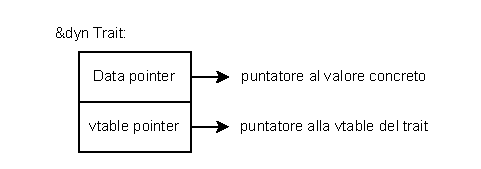
\includegraphics[width=0.8\textwidth]{Figures/vtable.drawio.pdf}
\end{figure}
Per mostrare la necessità di utilizzare i trait objects, consideriamo l' implementazione del design pattern \textit{Observer} \cite{gamma-design-patterns}: il \texttt{Subject} deve poter mantenere la collezione degli \texttt{Observer}, i quali vanno trattati in maniera uniforme nonostante possano essere di tipi diversi. Per fare ciò, definiamo il trait \texttt{Observer} e le sue implementazioni:
\begin{minted}[fontsize=\small]{Rust}
    trait Observer {
        fn update(&self, data: &str);
    }

    struct ConcreteObserverA;

    impl Observer for ConcreteObserverA {
        fn update(&self, data: &str) {
            println!("ConcreteObserverA received: {}", data);
        }
    }

    struct ConcreteObserverB;

    impl Observer for ConcreteObserverB {
        fn update(&self, data: &str) {
            println!("ConcreteObserverB received: {}", data);
        }
    }
\end{minted}
Ora, definiamo il \texttt{Subject} che mantiene una lista di \texttt{Observer} come trait objects:
\begin{minted}[fontsize=\small]{Rust}
    struct Subject {
        observers: Vec<Box<dyn Observer>>,
    }

    impl Subject {
        fn new() -> Self {
            Subject {
                observers: Vec::new(),
            }
        }

        fn add_observer(&mut self, observer: Box<dyn Observer>) {
            self.observers.push(observer);
        }

        fn notify_observers(&self, data: &str) {
            for observer in &self.observers {
                observer.update(data);
            }
        }
    }
\end{minted}
Quando si usa un trait object, Rust deve utilizzare il dynamic dispatch: il compilatore non conosce tutti i tipi che possono essere utilizzati nel codice che sta utilizzando il trait object, quindi non sa quale metodo implementato su quale tipo chiamare. La risoluzione della chiamata avviene a runtime tramite la vtable associata al trait object, con un'operazione a complessità costante.
\subsection{Java}
In Java, il meccanismo di risoluzione dei metodi è strettamente legato al concetto di ereditarietà e polimorfismo. Al fine della trattazione, definiamo un metodo virtuale come un metodo di istanza che può essere sovrascritto. Quindi metodi dichiarati come \texttt{static}, \texttt{final} o \texttt{private} non sono considerati virtuali. Java segue la seguente semantica di invocazione di metodi:
\begin{itemize}
    \item Se il metodo non è virtuale, la risoluzione avviene completamente a compile-time.
    \item Se il metodo è virtuale, la scelta dell'implementazione del metodo avviene a runtime. Questo avviene attraverso una vtable in maniera simile a Rust. Anche in questo caso si ottiene la selezione del metodo con complessità costante.
\end{itemize} 
In Java, tutte le chiamate a metodi non virtuali sono risolte a compile-time in maniera simile a come Rust risolve le chiamate di funzione. Questo significa che il compilatore sa esattamente quale metodo chiamare e non è necessario alcun meccanismo di dispatch a runtime. In particolare, per ottenere il comportamento di una funzione Rust si utilizza la keyword \texttt{static} che permette di definire metodi che appartengono alla classe stessa piuttosto che a una specifica istanza della classe. Ad esempio, considerando il listato \ref{lst:rust_function_call}, l'equivalente in Java sarebbe:
\begin{minted}[fontsize=\small]{Java}
    public class Main {
        public static int plusOne(int x) {
            return x + 1;
        }

        public static void main(String[] args) {
            int result = plusOne(5);
            System.out.println("The result is: " + result);
        }
    }
\end{minted}
Il caso più interessante è quello delle chiamate a metodi virtuali. Un metodo virtuale può essere sovrascritto in una sottoclasse per fornire una nuova implementazione, si parla di \textit{overriding}. In particolare, affinché avvenga l'overriding, si devono realizzare due condizioni:
\begin{itemize}
    \item Il metodo della sottoclasse deve avere lo stesso nome del metodo della superclasse.
    \item Il metodo della sottoclasse deve avere gli stessi parametri, cioè lo stesso numero, tipo e ordine degli argomenti; il tipo di ritorno deve essere lo stesso o un sottotipo (covarianza del tipo di ritorno).
\end{itemize}
In generale, il compilatore Java vede solo il riferimento statico di una variabile, ma non vede il tipo effettivo dell'oggetto a cui punta: questa informazione diventa disponibile solo durante l'esecuzione. Quando un metodo virtuale viene chiamato, l'implementazione del metodo da utilizzare è determinata a runtime in base al tipo effettivo su cui il metodo viene chiamato e sulla firma del metodo. Il \textit{Dynamic Method Lookup} è il processo tramite cui la JVM determina quale implementazione del metodo chiamare per una determinata firma. Ad esempio:
\begin{minted}[fontsize=\small]{Java}
    class Vehicle {
        public void start() {
            System.out.println("Vehicle is starting");
        }
    }
    class Car extends Vehicle {
        @Override
        public void start() {
            System.out.println("Car is starting");
        }
    }

    class Motorcycle extends Vehicle {
        @Override
        public void start() {
            System.out.println("Motorcycle is starting");
        }
    }

    public static void main(String[] args) {
        Vehicle[] vehicles = {new Car(), new Motorcycle()};
        for (Vehicle v : vehicles) {
            v.start(); // Chiamata a metodo virtuale
        }
    }
\end{minted}
L'invocazione di \texttt{start()} è risolta a runtime tramite dynamic method lookup, in base al tipo effettivo dell'oggetto a cui il riferimento \texttt{v} punta. Quindi l'esecuzione del metodo \texttt{main} produce il seguente output:
\begin{verbatim}
    Car is starting
    Motorcycle is starting
\end{verbatim}
In particolare, se un metodo virtuale non viene sovrascritto in una sottoclasse, la chiamata al metodo utilizza l'implementazione della superclasse. Questo viene ripetuto ricorsivamente lungo la gerarchia delle classi fino a trovare un'implementazione del metodo. 

Java offre anche un meccanismo di polimorfismo statico tramite il concetto di \textit{Method Overloading}, ossia la definizione di più metodi con lo stesso nome ma firme diverse (diverso numero o tipo di parametri) all'interno di una classe. La risoluzione della chiamata a un metodo in overload avviene a compile-time in base al tipo statico sia dell'oggetto su cui viene chiamato, che degli argomenti con cui il metodo viene chiamato. Ad esempio:
\begin{minted}[fontsize=\small]{Java}
    public class Calculator {
        public int add(int a, int b) {
            return a + b;
        }

        public double add(double a, double b, double c) {
            return a + b + c;
        }
    }

    public static void main(String[] args) {
        Calculator calc = new Calculator();

        // Chiama add(int, int)
        System.out.println(calc.add(2, 3));  

        // Chiama add(double, double, double)
        System.out.println(calc.add(1.5, 2.5, 3.5)); 
    }
\end{minted}
Rust non supporta l'overloading dei metodi nel senso di Java, però è possibile avere metodi con lo stesso nome, volendo anche la stessa firma, per uno stesso tipo tramite l'uso di blocchi \texttt{impl} nel seguente modo:
\begin{minted}[fontsize=\small]{Rust}
    struct Calculator;

    trait Adder {
        fn add(&self, a: i32, b: i32) -> i32;
    }

    impl Calculator {
        fn add(&self, a: i32, b: i32) -> i32 {
            a + b
        }
    }

    impl Adder for Calculator {
        fn add(&self, a: i32, b: i32) -> i32 {
            // Implementazione diversa per il trait
            // ad esempio con operazioni bitwise            
        }
    }
\end{minted}
Se si crea un'istanza di \texttt{Calculator} e si chiama il metodo \texttt{add}:
\begin{minted}[fontsize=\small]{Rust}
    fn main() {
        let calc = Calculator;
        let result = calc.add(2, 3);
        println!("Result: {}", result); // Chiama Calculator::add
    }
\end{minted}
Il metodo chiamato è quello definito direttamente su \texttt{Calculator}, poiché il compilatore dà priorità ai metodi innati della struct, ossia quelli definiti nel blocco \texttt{impl} della struct stessa, rispetto ai metodi forniti da un trait implementato dalla struct. In generale, l'algoritmo di risoluzione è molto più complesso e possono verificarsi casi di ambiguità più sofisticati rispetto all'esempio appena visto, in cui il compilatore non riesce a determinare quale metodo chiamare. In questi casi, si deve sempre ricorrere alla fully qualified syntax \footnote{La sintassi per la fully qualified syntax è \texttt{<Type as Trait>::method(\&received, args...)}.} per risolvere l'ambiguità. Anche in Java si possono verificare ambiguità nel caso di overloading, ad esempio:
\begin{minted}[fontsize=\small]{Java}
    public interface A {}

    public interface B {}

    public class C implements A, B {}

    public class D {

        public void method(A a) { /* ... */ }
        public void method(B b) { /* ... */ }

        public static void main(String[] args) {
            // Errore di compilazione per ambiguità
            new D().method(new C());
        }

    }
\end{minted}
In questo caso, la chiamata a \texttt{method(new C())} genera un errore di compilazione per ambiguità, poiché \texttt{C} implementa sia \texttt{A} che \texttt{B}, e quindi non è chiaro quale versione di \texttt{method} debba essere chiamata. Per risolvere l'ambiguità, si può utilizzare un cast esplicito oppure modificare il codice per evitare la situazione ambigua, ad esempio definendo un nuovo metodo \texttt{method(C c)}.
\begin{comment}
Java mette a disposizione due meccanismi linguistici per ottenere metodi polimorfi:
\begin{itemize}
    \item \textit{Method Overloading}, che consente di definire più metodi con lo stesso nome ma firme diverse (diverso numero o tipo di parametri). 
    \item \textit{Method Overriding}, che consente a una sottoclasse di fornire una nuova implementazione di un metodo ereditato dalla superclasse. 
\end{itemize}
L'overloading è un meccanismo statico, questo significa che la firma del metodo da chiamare è scelta in fase di compilazione in base al tipo statico sia dell'oggetto su cui viene chiamato, che degli argomenti con cui il metodo viene chiamato.

L'overriding, invece, è un meccanismo dinamico: la scelta del metodo avviene a runtime in base al tipo effettivo dell'oggetto su cui il metodo viene chiamato. Questo permette di ottenere il comportamento polimorfo tipico della programmazione orientata agli oggetti. 
\end{comment}

\section{Estensione del comportamento in Java e Rust}
\label{sec:extending_behavior}
Considerando quanto detto nelle sezioni precedenti, in particolare le sezioni \ref{sec:structs} e \ref{sec:rust_traits}, si può notare una differenza sostanziale tra Java e Rust: in Java, una classe definisce tre diversi elementi:
\begin{itemize}
    \item Lo stato degli oggetti attraverso i campi.
    \item Il comportamento attraverso i metodi.
    \item Il tipo degli oggetti attraverso la gerarchia di classi e interfacce.
\end{itemize}
questo è molto diverso da quello che accade in Rust in cui questi tre elementi sono rappresentati nel seguente modo:
\begin{itemize}
    \item Lo stato e il tipo degli oggetti è definito dalle \texttt{struct}.
    \item Il comportamento è definito all'interno di un blocco \texttt{impl} che può essere associato a una \texttt{struct} o a un \texttt{trait}.
\end{itemize}
Quindi, in Java, stato e comportamento sono definiti insieme in una singola entità, la classe, mentre in Rust c'è una separazione di queste responsabilità. Questa differenza ha implicazioni significative su come si estende il comportamento di tipi esistenti in ciascun linguaggio. In particolare, poiché Rust non supporta l'ereditarietà tra tipi, e quindi nemmeno la ridefinizione dei metodi (overriding), l'estensione di comportamento deve essere ottenuta tramite composizione e implementazione di traits. 

Consideriamo il seguente scenario, ispirato al libro Core Java for the Impatient \cite{horstmann-java-impatient}: vogliamo modellare il caso in cui sia necessario calcolare lo stipendio di un dipendente all'interno di un'azienda. Questo può essere un semplice impiegato o un manager che riceve un bonus. Poiché un manager è un tipo speciale di impiegato, l'obiettivo è quello di riusare il codice che definisce il comportamento di un dipendente per estenderlo e adattarlo al caso specifico del manager. In Java, questo può essere fatto tramite meccanismi OOP come ereditarietà e overriding. In Rust, invece, si può utilizzare composizione e traits per ottenere un comportamento analogo. In Java, si può rappresentare un dipendente attraverso la classe \texttt{Employee}:
\begin{minted}[fontsize = \small]{Java}
    class Employee {
        private double salary;
        
        public double getSalary() {
            return salary;
        }
    }
\end{minted}
Ora, definiamo la classe \texttt{Manager} che estende \texttt{Employee} e ridefinisce il metodo \texttt{getSalary()}:
\begin{minted}[fontsize = \small]{Java}
    class Manager extends Employee {
        private double bonusPercentage;

        @Override
        public double getSalary() {
            return getSalary() * bonusPercentage;
        }
    }
\end{minted}
Si può notare che tramite ereditarietà, la sottoclasse \texttt{Manager} ha ereditato sia lo stato (campo \texttt{salary}) che il comportamento (metodo \texttt{getSalary()}) dalla superclasse \texttt{Employee}, e ha sovrascritto il metodo \texttt{getSalary()} per fornire un nuovo comportamento specifico per i manager. In Rust, si può utilizzare la composizione:
\begin{minted}[fontsize = \small]{Rust}
    struct Employee {
        salary: f64,
    }

    impl Employee {
        fn get_salary(&self) -> f64 {
            self.salary
        }
    }

    struct Manager {
        employee: Employee,
        bonus_percentage: f64,
    }

    impl Manager {
        fn get_salary(&self) -> f64 {
            self.employee.get_salary() * self.bonus_percentage
        }
    }
\end{minted}
Tramite questa implementazione, si può riutilizzare il codice di \texttt{Employee} all'interno di \texttt{Manager}: attraverso la composizione, \texttt{Manager} ha un campo che è un'istanza di \texttt{Employee}, e può chiamare il metodo \texttt{get\_salary()} di \texttt{Employee} per ottenere lo stipendio base, e poi calcolare il bonus.

Ora, consideriamo il caso in cui si voglia trattare \texttt{Manager} e \texttt{Employee} in maniera uniforme. In Java, questo è possibile grazie al fatto che \texttt{Manager} è un sottotipo di \texttt{Employee}, quindi si può usare il polimorfismo basato su sottotipi. Ad esempio, consideriamo la seguente classe Java:
\begin{minted}[fontsize = \small]{Java}
    class Payroll {
        public void paySalary(Employee emp) {
            double amount = emp.getSalary();
            System.out.println("Processing payment of: " + amount);
            // Logica di pagamento
        }
    }
\end{minted}
In questo caso, tramite il polimorfismo dinamico di Java, il metodo \texttt{paySalary()} può accettare sia istanze di \texttt{Employee} che di \texttt{Manager}, e chiamare il metodo corretto \texttt{getSalary()} in base al tipo effettivo dell'oggetto passato. In Rust, il codice precedente non permette questa flessibilità, poiché \texttt{Manager} ed \texttt{Employee} sono completamente scorrelati a livello di tipi. Per ottenere un comportamento simile in Rust, si può rifattorizzare il codice utilizzando i traits:
\begin{itemize}
    \item Definire un trait \texttt{Payable} che dichiara il metodo \texttt{get\_salary()}.
    \item Implementare il trait \texttt{Payable} per entrambe le strutture (\texttt{Employee} e \texttt{Manager}), spostando in questa implementazione la logica dei rispettivi metodi \texttt{get\_salary()}, che quindi non devono più essere definiti direttamente nelle strutture.
\end{itemize}
\begin{minted}[fontsize = \small]{Rust}
    trait Payable {
        fn get_salary(&self) -> f64;
    }

    impl Payable for Employee {
        fn get_salary(&self) -> f64 {
            self.salary
        }
    }

    impl Payable for Manager {
        fn get_salary(&self) -> f64 {
            self.employee.get_salary() * self.bonus_percentage
        }
    }
\end{minted}
Adesso \texttt{Employee} e \texttt{Manager} implementano entrambi il trait \texttt{Payable}, quindi si può definire una funzione che accetta un parametro generico con vincolo di tipo:
\begin{minted}[fontsize = \small]{Rust}
    struct Payroll;

    impl Payroll {
        fn pay_salary<T: Payable>(&self, emp: &T) {
            let amount = emp.get_salary();
            println!("Processing payment of: {}", amount);
            // Logica di pagamento
        }
    }
\end{minted}
In questo modo, la funzione \texttt{pay\_salary()} può accettare sia istanze di \texttt{Employee} che di \texttt{Manager}, e chiamare il metodo corretto \texttt{get\_salary()} in base al tipo effettivo dell'oggetto passato. Tuttavia, a differenza di Java, questa flessibilità viene ottenuta tramite l'uso di generics e trait, piuttosto che tramite relazioni di sottotipo. Inoltre, a differenza di Java, il meccanismo utilizzato da Rust è completamente statico, come visto nella sezione \ref{sec:generics}. 

Estendiamo ulteriormente l'esempio aggiungendo un nuovo metodo nella classe \texttt{Payroll}:
\begin{minted}[fontsize = \small]{Java}
    class Payroll {
        public void paySalary(Employee emp) { /* ... */ }

        public void payEmployees(List<Employee> employees) {
            for (Employee emp : employees) {
                paySalary(emp);
            }
        }
    }
\end{minted}
Ancora una volta, grazie al subtyping di Java, \texttt{payEmployees()} funziona correttamente. In Rust, limitarsi a usare generics non è sufficiente per ottenere lo stesso comportamento. Questo perché i generics vengono monomorfizzati, rendendo impossibile la creazione di una collezione di tipi eterogenei. Per ottenere questo comportamento in Rust, si deve utilizzare i trait object:
\begin{minted}[fontsize = \small]{Rust}
    impl Payroll {
        fn pay_salary(&self, emp: Box<dyn Payable>) {
            println!("Paying salary: {}", emp.get_salary());
        }

        fn pay_employees(&self, employees: Vec<Box<dyn Payable>>) {
            for emp in employees {
                self.pay_salary(emp);
            }
        }
    }
\end{minted}
In questo caso, tramite trait objects e dynamic dispatch, la funzione \texttt{pay\_employees()} può accettare una collezione di oggetti eterogenei che implementano il trait \texttt{Payable}, e chiamare il metodo \texttt{get\_salary()} corretto in base al tipo effettivo di ogni oggetto nella collezione. 

Da questo esempio si notare differenze sostanziali tra come i due linguaggi supportano l'estensione del comportamento. Non esiste un approccio migliore ma dipende dal contesto specifico e dai requisiti del progetto. In generale, si possono fare le seguenti osservazioni:
\begin{itemize}
    \item Java offre un meccanismo di estensione del comportamento più diretto e intuitivo tramite l'ereditarietà e il polimorfismo basato su sottotipi. Questo rende più semplice la creazione di gerarchie di classi e l'estensione del comportamento esistente. Invece, Rust, richiede molto più lavoro per ottenere lo stesso risultato. Rust sacrifica un po' di semplicità per ottenere una maggiore sicurezza e performance.
    \item Rust lascia allo sviluppatore più libertà di scelta riguardo l'utilizzo di meccanismi statici o dinamici. Questo anche perché Rust utilizza solamente static dispatch a meno che non sia dichiarato differentemente dallo sviluppatore tramite i trait objects. Java, invece, se utilizzato secondo i principi della programmazione orientata agli oggetti, utilizza principalmente il dynamic dispatch.
    \item La scelta della composizione è quasi obbligata in Rust, questo può essere visto come una cosa positiva perché l'estensione del comportamento tramite ereditarietà porta con sé diversi problemi quali:
    \begin{itemize}
        \item Il \textit{Fragile Base Class Problem} \cite{mikhajlov-sekerinski-fragile-base-class}: quando una superclasse viene modificata, le sottoclassi dipendenti da essa possono rompersi in modi inaspettati.
        \item Quando viene estesa una classe si ereditano tutti i suoi metodi (\texttt{public} e \texttt{protected}), anche quelli a cui non sono interessato, e non si può fare altrimenti. Questo può causare comportamenti indesiderati. Per risolvere questo problema si può nuovamente utilizzare il pattern \textit{Adapter} per adattare il comportamento della superclasse.
        \item La possibilità di estendere in maniera incontrollata le classi ha portato Java ad introdurre le classi (e interfacce) \texttt{Sealed} tramite le quali è possibile mettere dei vincoli su quali classi possono estendere una determinata superclasse.
    \end{itemize}
\end{itemize}
\begin{comment}
\section{Meccanismi di Dispatch}
Quando il codice coinvolge il polimorfismo, sono necessari meccanismi per determinare quale versione specifica di metodo sta venendo effettivamente eseguita. Questo processo prende il nome di \textit{dispatch}. Esistono due forme di dispatch: 
\begin{itemize}
    \item Lo \textit{Static Dispatch}, in cui la risoluzione della chiamata viene risolta a tempo di compilazione.
    \item Il \textit{Dynamic Dispatch}, in cui la risoluzione della chiamata avviene a run-time. 
\end{itemize}
%TODO Inserire un piccolo confronto pro/contro per s/d dispatch

\subsection{Static Dispatch}
In Rust, il meccanismo di static dispatch viene realizzato attraverso \textit{generics} e i \textit{trait bounds}. Quando si utilizza un tipo generico con un trait bound, il compilatore genera una versione specializzata della funzione per ogni tipo concreto utilizzato. Questo processo è noto come \textit{monomorphization} (descritto in dettaglio nella Sezione \ref{sec:generics}). Per mostrare esplicitamente come lo static dispatch venga implementato in Rust consideriamo il seguente codice:
\begin{minted}[fontsize=\small] {Rust}
    trait Drivable {
        fn drive(&self);
    }

    struct Car;
    impl Drivable for Car {
        #[inline(never)]
        fn drive(&self) {
            println!("You are driving a car.");
        }
    }

    struct Motorcycle; 
    impl Drivable for Motorcycle {
        #[inline(never)]
        fn drive(&self) {
            println!("You are driving a motorcycle.");
        }
    }

    struct Boat;
    impl Drivable for Boat {
        #[inline(never)]
        fn drive(&self) {
            println!("You are driving a boat");
        }
    }
\end{minted}
Definiamo la seguente funzione generica con vincolo di tipo:
\begin{minted}[fontsize = \small]{Rust}
    fn static_dispatch<T: Drivable>(t: T) {
        t.drive();
    }
\end{minted}
Ora, all'interno del nostro \texttt{main()} chiamiamo \texttt{static\_dispatch()} con uno dei tre tipi concreti precedentemente definiti:
\begin{minted}[fontsize = \small]{Rust}
    fn main() {
        static_dispatch(Car{});
        static_dispatch(Motorcycle{});
        static_dispatch(Boat{});
    }
\end{minted}
Durante la compilazione, tramite monomorphization, verranno create tre copie della funzione \texttt{static\_dispatch()}: una per ogni tipo con cui è stata chiamata. Questo si può vedere utilizzando i seguenti comandi\footnote{Il primo comando compila il file Rust senza ottimizzazioni e con informazioni di debug dettagliate. Questo è necessario per produrre un eseguibile "leggibile" e completo per il debug. Il secondo comando utilizza LLDB, un debugger per linguaggi come C e Rust, per disassemblare la funzione \texttt{drive} e mostrare i suoi indirizzi di memoria.} dal terminale:
\begin{minted}[fontsize=\small]{bash}
rustc -C opt-level=0 -C debuginfo=2 main.rs
lldb ./main --batch -o "disassemble --name drive" > disassembly.txt
\end{minted}
Il comando genera un file \texttt{disassembly.txt} contenente la disassemblazione delle funzioni \texttt{drive} con i vari tipi, mostrando chiaramente che ogni funzione ha un indirizzo di memoria distinto:

\begin{verbatim}
Car::drive        -> 0x100000a2c
Motorcycle::drive -> 0x100000a64
Boat::drive       -> 0x100000a9c
\end{verbatim}

Questo evidenzia come lo static dispatch risolva la chiamata alla funzione al momento della compilazione, senza alcun overhead a runtime. 

In Java, lo \textit{static dispatch} è realizzato tramite il \textit{method overloading}. In questo meccanismo, più metodi condividono lo stesso nome ma differiscono per la lista dei parametri (numero o tipo). La scelta del metodo corretto viene risolta dal compilatore in base ai tipi statici degli argomenti.

Consideriamo il seguente esempio:

\begin{minted}[fontsize=\small]{java}
public class StaticDispatch {
		
    public double sum(int op1, int op2) {
        return op1 + op2;
    }
	
    public double sum(double op1, double op2) {
        return op1 + op2;
    }
	
    public static void main(String[] args) {
        double x = new StaticDispatch().sum(1, 1);
        double y = new StaticDispatch().sum(1.0, 1.0);
    }
}
\end{minted}

In questo caso, abbiamo due metodi omonimi \texttt{sum}, rispettivamente con parametri di tipo \texttt{int} e \texttt{double}. Durante la compilazione, la chiamata \texttt{sum(1, 1)} viene risolta come invocazione del metodo \texttt{sum(int, int)}, mentre la chiamata \texttt{sum(1.0, 1.0)} come invocazione del metodo \texttt{sum(double, double)}.  

Per osservare cosa accade a livello di bytecode, compiliamo ed utilizziamo il comando:

\begin{minted}[fontsize=\small]{bash}
    javac .\StaticDispatch.java
    javap -c .\StaticDispatch.class > bytecode.txt
\end{minted}

L'output (semplificato) scritto sul file \texttt{bytecode.txt} è il seguente:
\begin{verbatim}
  public static void main(int[]);
    Code:
       0: new           #7    
       3: dup
       4: invokespecial #9    // Method "<init>":()V
       7: iconst_1
       8: iconst_1
       9: invokevirtual #10   // Method sum:(II)D
      12: dstore_1
      13: new           #7    
      16: dup
      17: invokespecial #9    // Method "<init>":()V
      20: dconst_1
      21: dconst_1
      22: invokevirtual #14   // Method sum:(DD)D
      25: dstore_3
      26: return
\end{verbatim}

Possiamo notare che:
\begin{itemize}
    \item Alla riga 9, \texttt{invokevirtual \#10} corrisponde a \texttt{sum:(II)D}, ovvero il metodo con parametri \texttt{int}.
    \item Alla riga 22, \texttt{invokevirtual \#14} corrisponde a \texttt{sum:(DD)D}, ovvero il metodo con parametri \texttt{double}.
\end{itemize}

Queste informazioni provengono dal \textit{constant pool} \footnote{La constant pool contiene le costanti necessarie per l'esecuzione del codice di una specifica classe. In pratica, è una struttura dati a runtime simile a una tabella dei simboli.} del bytecode, dove il compilatore ha già registrato a quale firma di metodo corrisponde ciascuna chiamata. In altre parole, nonostante entrambe le invocazioni utilizzino l'istruzione \texttt{invokevirtual}, a runtime la JVM non ha bisogno di fare alcuna ricerca aggiuntiva: la firma è già stata scelta a compile-time in maniera univoca.

Sebbene in entrambi i linguaggi si parli di \textit{static dispatch}, i meccanismi adottati sono profondamente diversi. In Rust, lo static dispatch si traduce in specializzazione del codice (funzioni distinte generate dal compilatore). In Java, invece, lo static dispatch si traduce in selezione della firma corretta (una voce distinta nel constant pool per ogni metodo). In entrambi i casi, la risoluzione avviene a compile-time e non vi è alcun overhead di dispatch a runtime. 
\subsection{Dynamic Dispatch}
Il meccanismo di generics e trait bounds appena descritto è adatto solamente quando si lavora con tipi omogenei di cui si conosce  il tipo esatto a compile-time. Tuttavia, quando si desidera lavorare con tipi eterogenei o quando il tipo esatto non è noto fino a runtime, è necessario utilizzare il \textit{dynamic dispatch}. 

Il dynamic dispatch in Rust viene realizzato attraverso l'uso di \textit{trait objects}. Un trait object è un puntatore a un tipo che implementa un determinato trait, consentendo di chiamare metodi definiti nel trait senza conoscere il tipo concreto a compile-time. Un trait object si definisce con la sintassi \texttt{Box<dyn Trait>}\footnote{Al posto di \texttt{Box<>} si può utilizzare qualsiasi altro tipo di puntatore. Questo è richiesto perché il compilatore di Rust deve sapere a compile time la dimensione della variabile.}, dove \texttt{Trait} è il trait che si desidera utilizzare. Ad esempio, consideriamo l'implementazione del design pattern Observer: il \texttt{Subject} deve poter mantenere la collezione degli \texttt{Observer}, i quali vanno trattati in maniera uniforme nonostante possano essere di tipi diversi. Per fare ciò, definiamo il trait \texttt{Observer} e le sue implementazioni:
\begin{listing}[H]
    \begin{minted}[fontsize=\small]{Rust}
        trait Observer {
            fn update(&self, data: &str);
        }

        struct ConcreteObserverA;

        impl Observer for ConcreteObserverA {
            fn update(&self, data: &str) {
                println!("ConcreteObserverA received: {}", data);
            }
        }

        struct ConcreteObserverB;

        impl Observer for ConcreteObserverB {
            fn update(&self, data: &str) {
                println!("ConcreteObserverB received: {}", data);
            }
        }
    \end{minted}
    \caption{Implementazione degli Observer.}
    \label{lst:observer}
\end{listing}
Ora, definiamo il \texttt{Subject} che mantiene una lista di \texttt{Observer} come trait objects:
\begin{minted}[fontsize=\small]{Rust}
    struct Subject {
        observers: Vec<Box<dyn Observer>>,
    }

    impl Subject {
        fn new() -> Self {
            Subject {
                observers: Vec::new(),
            }
        }

        fn add_observer(&mut self, observer: Box<dyn Observer>) {
            self.observers.push(observer);
        }

        fn notify_observers(&self, data: &str) {
            for observer in &self.observers {
                observer.update(data);
            }
        }
    }
\end{minted}
Rust implementa il dynamic dispatch tramite una \textit{vtable}. Essenzialmente, una vtable è una struttura generata dal compilatore che contiene puntatori a funzione. In particolare, un trait object è rappresentato internamente come una coppia di puntatori: 
\begin{itemize}
    \item Un puntatore alla vtable corrispondente alla combinazione tra il tipo concreto e il trait implementato.
    \item Un puntatore ai dati del tipo concreto.
\end{itemize}
\begin{figure}[H]
    \centering
    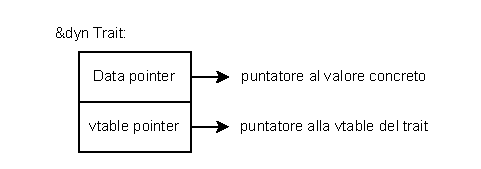
\includegraphics[width=0.8\textwidth]{Figures/vtable.drawio.pdf}
\end{figure}
Va notato che la vtable non è generata per il trait in generale, ma per ciascuna combinazione di tipo concreto e trait implementato. Considerando il listato \ref{lst:observer}, per ogni tipo che implementa il trait \texttt{Observer}, il compilatore genera una vtable separata: quindi sarà presente una vtable per la coppia (\texttt{ConcreteObserverA, Observer}) e una per (\texttt{ConcreteObserverB, Observer}). Quando, all'interno del metodo \texttt{notify\_observers()}, viene chiamato il metodo \texttt{update()} su un trait object, Rust esegue i seguenti passi:
\begin{itemize}
    \item Recupera il puntatore alla vtable del tipo concreto (tranne per \texttt{Object}).
    \item Utilizza il puntatore alla vtable per trovare l'indirizzo della funzione \texttt{update()}.
    \item Chiama la funzione \texttt{update()} passando il puntatore ai dati del tipo concreto.
\end{itemize}
Questo processo consente a Rust di determinare a runtime quale implementazione del metodo chiamare, basandosi sul tipo concreto dell'oggetto. 

In Java, il meccanismo di dynamic dispatch è implementato tramite il \textit{method overriding}, ossia la possibilità di ridefinire un metodo in una sottoclasse. Come in Rust, il metodo da chiamare viene determinato a runtime in base al tipo concreto dell'oggetto. Ogni classe presente in un'applicazione Java ha un'area di memoria all'interno della JVM che contiene metadati riguardanti quel tipo. All'interno di questa area sono contenuti due elementi fondamentali:
\begin{itemize}
    \item Un puntatore alla superclasse.
    \item Un puntatore alla vtable corrispondente al tipo concreto. Questa è simile alla vtable Rust, ossia un puntatore alla tabella dei metodi della classe.
\end{itemize}
In generale, quando viene chiamato un metodo su un oggetto tramite \texttt{invokevirtual}, la JVM consulta la vtable del tipo concreto per determinare quale implementazione del metodo chiamare. Se non esiste una definizione per quel metodo allora la JVM segue il puntatore alla superclasse e riprova finché non viene trovata la definizione del metodo chiamato. 

Per rendere più efficiente l'invocazione dei metodi, le vtable sono organizzate in modo da ridurre al minimo l'overhead dovuto all' attraversamento della gerarchia delle classi. In particolare:
\begin{itemize}
    \item I metodi definiti nella superclasse vengono inseriti nella vtable della sottoclasse nello stesso ordine in cui compaiono nella superclasse.
    \item I nuovi metodi, cioè quelli non presenti nella superclasse, vengono aggiunti in coda alla vtable.
\end{itemize}
Di conseguenza, quando una sottoclasse ridefinisce un metodo, questo mantiene la stessa posizione occupata nella vtable della superclasse, evitando ricerche aggiuntive. Ad esempio, consideriamo la seguente gerarchia di classi:
\begin{figure}[H]
    \centering
    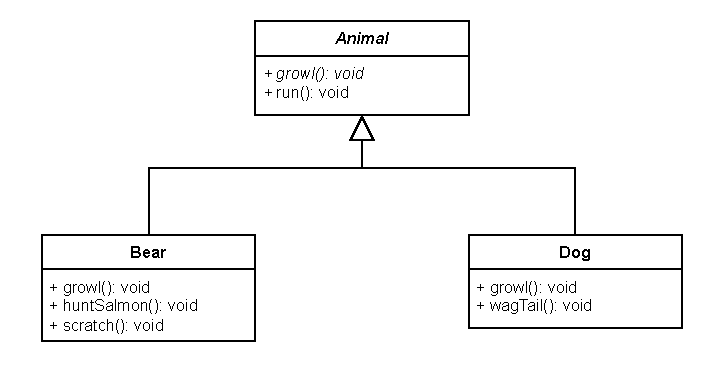
\includegraphics[width=1\textwidth]{Figures/uml1.drawio.pdf}
\end{figure}
Questa produce le seguenti vtable:
\begin{figure}[H]
    \centering
    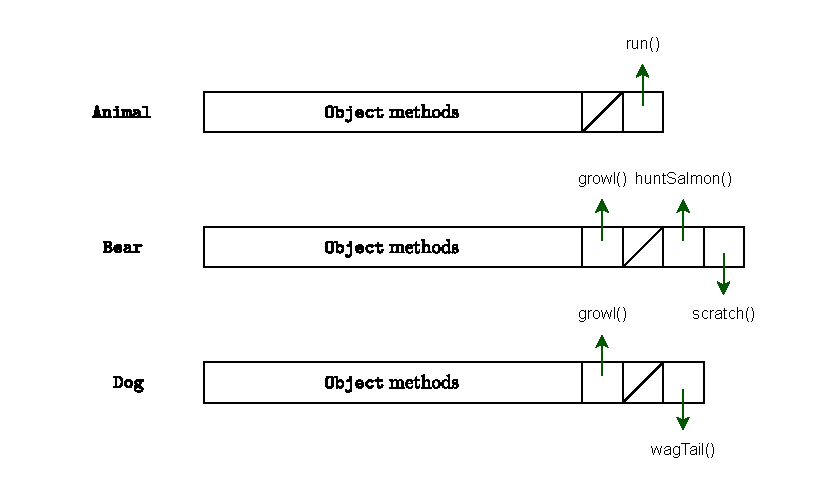
\includegraphics[width=\textwidth]{Figures/vtable1.drawio.pdf}
    \caption{Esempio di vtable in Java.}
    \label{fig:vtable_java}
\end{figure}
Considerando le vtable mostrate in Figura \ref{fig:vtable_java}, quando viene chiamato il metodo \texttt{Bear::run}, la JVM non troverà il metodo sovrascritto nella vtable di \texttt{Bear}, ma seguirà il puntatore alla superclasse \texttt{Animal} dove il metodo è definito \footnote{La prima volta che viene chiamato \texttt{Bear::run} la JVM memorizza il suo indirizzo nella vtable di \texttt{Bear}. In questo modo si migliora la performance delle chiamate successive.}. Nel caso di una gerarchia di classi più profonda, la ricerca potrebbe richiedere più passaggi e diventare più costosa. Da notare che questo sistema funziona solamente perché Java supporta l'ereditarietà singola per le classi: c'è solo un'unica superclasse diretta per ogni tipo (tranne che per \texttt{Object}). 

In conclusione, sia Rust che Java implementano il dynamic dispatch tramite l'uso di vtable, ma con alcune differenze chiave che riflettono i diversi approcci dei due linguaggi al polimorfismo:
\begin{itemize}
    \item In Rust, le vtable sono generate per ogni combinazione di tipo concreto e trait implementato. In Java, invece, ogni classe ha una singola vtable che include tutti i metodi ereditati e quelli definiti nella classe stessa.
    \item In Rust, il dynamic dispatch richiede l'uso esplicito di trait objects (ad esempio \texttt{Box<dyn Trait>}), mentre in Java il dynamic dispatch avviene automaticamente quando si chiama un metodo su un riferimento di tipo superclasse o interfaccia.
    \item Teoricamente, il dynamic dispatch in Rust ha un overhead ridotto rispetto a Java. Questo perché in Rust la vtable viene consultata direttamente per trovare l'indirizzo del metodo, mentre in Java potrebbe essere necessario attraversare la gerarchia delle classi per trovare la definizione del metodo.     
\end{itemize}
\end{comment}